\documentclass[12pt]{report}
\usepackage{listings}
\usepackage{amsmath}
\usepackage{amsfonts}
\usepackage{amssymb}
\usepackage{fancyhdr}
\usepackage{hyperref}
\usepackage[acronym]{glossaries}
\usepackage{graphicx}
\usepackage{wrapfig}
\usepackage{listings}
\usepackage{minted}
\usepackage{caption}
\usepackage{emptypage}
\usepackage{mathptmx}
\usepackage{setspace}
\usepackage{titlesec}
\usepackage[margin=1.5in,topmargin=0.5in]{geometry}
\usepackage{inconsolata}
%\usepackage{nopageno}

\titleformat{\chapter}[display]
    {\normalfont\huge\bfseries}{\chaptertitlename\ \thechapter}{20pt}{\Huge}
\titlespacing*{\chapter}{0pt}{0pt}{30pt}
%\makeglossaries

\pagestyle{fancy}
\fancyhead[C]{}
\fancyhead[L]{}
\fancyhead[R]{\it Adding Semantics to RESTful Web Services}

\fancyfoot[L]{\it Department of Computer Science \& Engineering, CET 2013}
\fancyfoot[C]{}
\fancyfoot[R]{\thepage}


\begin{document}
\begin{titlepage}
\begin{center}
{\huge {\bf Adding Semantics To RESTful Web Services}}\\
%{\huge \textbf{Omnipresent and Obsolete}}\\
\vspace{10mm}
{\it \textbf{Submitted in partial fulfillment for the award of the Degree of Bachelor of Technology in Computer Science and Engineering}}\\
\vspace{20mm}
{\it Submitted By:}\\
{\bf ABIL N GEORGE (09400002)}\\
{\bf AKHIL PM (09400005)}\\
{\bf DEEPAK KRISHNAN N (09400011)}\\
{\bf DHANANJAY BALAN (09400012)}\\

\vspace{5mm}
{\it Under the guidance of:}\\
{\bf DR. ABDUL NIZAR}\\
\vspace{30mm}

\includegraphics[width=0.3\textwidth]{images/cet_logo.jpg}\\
\vspace{3mm}
\textsc{\textbf{DEPARTMENT OF COMPUTER SCIENCE AND ENGINEERING}}\\
\vspace{1mm}
\textsc{\textbf {COLLEGE OF ENGINEERING}}\\
\vspace{1mm}
\textsc{\textbf{THIRUVANANTHAPURAM 16}}\\
\vspace{4mm}
\textbf{May, 2013}
\end{center}
\end{titlepage}


% Certificate and Acknow.
\newpage
\thispagestyle{empty}
\begin{center}
\textsc{{\textbf{DEPARTMENT OF COMPUTER SCIENCE AND ENGINEERING}}}\\
\vspace{1mm}
\textsc{\textbf{COLLEGE OF ENGINEERING}}\\
\vspace{1mm}
\textsc{\textbf{THIRUVANANTHAPURAM 16}}\\
\vspace{6mm}

\includegraphics[width=0.3\textwidth]{images/cet_logo.jpg}\\
\vspace{10mm}

\textbf{CERTIFICATE}
\vspace{4mm}
\end{center}
\begin{spacing}{1.5}
This is to certify that the project report entitled {\bf "Adding Semantics to RESTful Web Services"} is a bonafide record of the project work done by {\it Dhananjay Balan,Abil N George, Akhil PM, Deepak Krishnan}  under my supervision and guidance, in partial fulfillment for the award of the degree of {\bf Bachelor of Technology in Computer Science and Engineering} of the {\bf University of Kerala} during the year {\bf 2013}.\\
\end{spacing}
\vspace{5mm}
\noindent{Guide\hfill Head of the Department}\\
\vspace{8mm} \\
\noindent{\bf Dr. Abdul Nizar M, \hfill \bf Prof. Ajeena Beegom  A.S} \\
\noindent{Professor(Guide) \hfill Head of Department} \\
\noindent{Department Of Computer Science \hfill Department Of Computer Science} \\
\noindent{and Engineering \hfill and Engineering} \\
\noindent{College Of Engineering \hfill College Of Engineering} \\
\noindent{Trivandrum-16 \hfill Trivandrum-16} \\

% Ack
\newpage
\thispagestyle{empty}
\begin{center}
\textsc{\bf ACKNOWLEDGMENT}
\end{center}
\vspace{20mm}
\begin{spacing}{1.5}
First and foremost, we wish to place on records our ardent and earnest gratitude to our project guide {\bf Dr. Abdul Nizar, Professor, Department of Computer Science and Engineering}. His tutelage and guidance was the leading factor in translating our efforts to fruition. His prudent and perspective vision has shown light on our trail to triumph.

We are extremely happy to mention great word of gratitude to {\bf Prof. Ajeena Beegom A.S, Head of the Department of Computer Science and Engineering} for providing us with all facilities of this work.

Finally yet importantly,we would like to express our gratitude to our project coordinator {\bf Mrs. Deepa S.S}, for her valuable assistance provided during the course of the project.

We would also extend our gratefulness to all the staff members in the Department. We also thank all our friends and well-wishers who greatly helped us in our endeavour.
.\\
\end{spacing}
\vspace{15mm}
{\raggedleft {\bf Abil N George \\ Akhil P M \\ Deepak Krishnan N \\ Dhananjay Balan\\}}
\begin{abstract}
\begin{spacing}{1.5}
Development of a semantic web is gaining a lot of traction recently. At the same time, another change is also getting a lot popular on the web - a move from complex SOAP based web services to the simpler RESTful services that work over the existing HTTP infrastructure. RESTful services were born out of an attempt to unify and simplify the creation and consumption of web based services, and to increase its adoption. Adding semantics to web service descriptions is an important step towards a better web that is accessible to both humans and machines alike. With the web taking a definite turn towards RESTful web services from the traditional RPC- like SOAP based services, it is important to devise a semantic description method for such services. However, for these solutions to be really adopted by developers, they should adhere to the RESTful philosophy and provide a low entry barrier. The proposed solution aligns with the REST philosophy and architecture and reuses existing service documentations to double them as machine-readable descriptions. The Microformats-like syntax used by the solution is simple and easy to write and maintain from a developer perspective. Further, the language describes services as resources with attributes instead of using an RPC-like input-operation-output concept used by most of the current solutions. This markup syntax is then extended to add interlinking between RESTful services, enabling automatic discovery and composition of services. The solution should further reduce the entry barrier for developers and thus increase adoption, resulting in a widely accepted standard. The existence of such a standard technique can make the wealth of resources available on the Internet accessible to machines, enabling the creation of intelligent software agents that can get a lot of work done with no to minimal intervention from humans. 
\end{spacing}
\end{abstract}

\newpage
{
\pagestyle{empty}
\pagenumbering{roman}
\tableofcontents
\listoffigures
\listoftables
\cleardoublepage
}

\pagestyle{fancy}
\pagenumbering{arabic}
\chapter{INTRODUCTION}
\begin{spacing}{1.5}
Semantic web is a collective movement towards adding semantics or meaning to the data available on the internet thus making them machine readable. Data with semantics will be key in the future web where human interaction can be reduced for exploring and using this information. While the vision of a Semantic Web has been around for more than fifteen years it still has a long way to go before mainstream adoption will be achieved. One of the reasons for that is, the fear of average Web developers to use Semantic Web technologies. The reasons for this are manifold and should be further researched. Some developers are overwhelmed by the (perceived) complexity or think they have to be AI experts to make use of the Semantic Web and simply shut down when they hear the word Ontology. Others are still  waiting for a killer application making it a classical chicken- and-egg problem. A common perception is that the Semantic Web is a disruptive technology which makes it a show-stopper for enterprises needing to evolve their systems and build upon existing infrastructure investments. Obviously some developers are also just reluctant to use new technologies. 

There have been two main initiatives towards adding semantics to the web: Linked Data and semantic annotations. 

Linked Data is an effort to create a web of data, parallel to the web of documents - the web we know and use today\cite{1}. Since HTML, the language of the web was deemed insufficient to accurately and expressively describe strongly typed relationships between data, a new XML based language named RDF (Resource Description Framework) was suggested\cite{2}. RDF documents define relationships in the form of subject-predicate-object triplets and can thus model a wide variety of links. RDF documents are supported by schemas written in either RDFS\cite{3}or OWL\cite{4}\cite{5}.

While Linked Data is very expressive when it comes to describing relationships, it has a downside as well: these descriptions are separate from the current web that humans use and leaves developers with another artifact to develop and maintain. This has lead into development of techniques that try to integrate the human web and the machine-readable web into one single entity. Two important standards developed in the area of semantic annotations are Microformats\cite{6},RDFa\cite{7}\cite{8} and SEREDASj\cite{14}. 

\section{Semantic Web Services} 
The concept of semantic web has also been applied to web services, using semantic web techniques to 
\begin{itemize}
\item Describe web services themselves and
\item Add meaning to the results provided by web services to make them machine 
readable and to increase the utility of the information gathered. 
\end{itemize}

Most of the research in semantic web services has been around SOAP based services. These are the "conventional" web services that have been the prime solution until a few years back. While SOAP packs a lot of power into accurately describing various aspects of a service, such verbosity is often undesired and leaves developers with a high entry-barrier that most chose not to take. 

The recent attention gained by RESTful services\cite{9} – an entirely different service architecture - is a natural response to the prohibitive complexity of developing and describing SOAP based services. The REST philosophy prioritizes simplicity over verbosity and works over the existing HTTP infrastructure. Resources are represented as URLS and CRUD operations are defined by the POST, GET, PUT and DELTE HTTP methods respectively. Its resemblance to the way the web works has resulted in widespread adoption since the days of Web 2.0.

The major problem of RESTful services is that no agreed machine-readable description format exists to document them. All the required information of how to invoke them and how to interpret the various resource representations is communicated out-of-band by human-readable documentations. This usually does not cause any problems in the human Web since humans inherently understand the representations and are thus able to quickly adapt to new control flows (e.g: a change in the order sequence or a new login page to access the service). Machines on the other hand have huge problems to understand such representations; just as disabled users sometimes have. A blind user for instance cannot make any use of information contained in graphics. Machines suffer even more from such usability and accessibility problems. 

Currently machine-to-machine communication is often based on static knowledge and tight coupling to resolve those issues. The challenge is thus to bring some of the human Web‘s adaptivity to the Web of machines to allow the building of loosely coupled, reliable, and scalable systems. After all, a Web service can be seen as a special Web page meant to be consumed by an autonomous program as opposed to a human being. The Web already supports machine-to-machine communication, what‘s not machine-processable about the current Web is not the protocol (HTTP), it is the content. 

Some research has gone into utilizing semantic web techniques specifically for RESTful services. These solutions suffer from either of the two problems. 

\begin{itemize}
\item They are generalizations of existing mechanisms to describe SOAP services. REST being an entirely different architecture, such an approach results in a lot of unwanted markup and code. This conversion to another architecture steals some of the implicit properties of RESTful architecture like simplicity, focus on resources rather than services etc.
\item These solutions require an external description, which has to be created and maintained by the developer adding to the effort required. 
\end{itemize}

Further, the solutions for describing RESTful services do not take into account the possibilities of automatic discovery and composition of services. Papers had been published on new proposals that work together with one of these markup languages to provide description. However, these solutions usually suffer from the same issues as the markup languages - they are mainly aimed at SOAP based services and do not fit well into the REST architecture.
\end{spacing}

\chapter{SCOPE OF THE PROJECT}
\begin{spacing}{1.5}

The main feature of this new approach is the automation of mashup creation. It enables automatic  discovery and composition of services.The existence of such a standard technique can make the wealth of resources available on the Internet accessible to machines, enabling the creation of intelligent software agents that can get a lot of work done with no to minimal intervention from humans.

The process of creating mashups is a manual task  which require a lot of human interaction with the existing standards. There exists  two popular mashup creators ;Yahoo Pipes\cite{pip} and IFTTT\cite{ift}.

Yahoo pipes is a free online service to aggregate,manipulate and mashup content from around the web. Modules can be dragged onto its interface and link between them by connecting output of one service as input to other services. It is developed to assist non-technical users to create mashups. You can create your own custom RSS feeds  with Yahoo Pipe that pull in content from a variety of sources and filter it so that you only see the most relevant news stories. It requires no plugins or coding.

However Yahoo Pipes faces many drawbacks. It cannot create a mashup between any pair  of services. It works well with a defined set of web services like RSS feeds etc. Pipes is being very buggy lately and has stopped saving new pipes these days. Also  some times it is very slow in working. A typical operation with Yahoo Pipes takes atleast 200 ms. Fetching an RSS feed with a filter will normally take 400 ms in Yahoo Pipe. Also Yahoo Pipes lack processing power and cannot works well with website from far east. It fails to generate results while processing complex regex from far multiple locations, with hundreds of posts every minutes.

IFTTT is a service that lets you create powerful connections with one simple statement: {\it “if this then that “}.The “this” part of a recipe is a trigger. The that part of a recipe is an action. The combination of a trigger and an action from a customer's active channels are called recipes. Pieces of data from trigger a are called Ingredients. The service offers triggers and actions for 61 channels such as Twitter,Foursquare,Flickr and Box etc.

There are two types of recipes, Personal recipes and shared recipes. Personal Recipes are a combination of a Trigger and an Action from your active Channels.Personal Recipes can be turned on and off. When turned back on, they pick up as if you had just created them. Personal recipes check for new trigger data every 15 minutes. Shared recipes are useful templates shared by the IFTTT community. By combining IFTTT with other services such as Yahoo Pipes  one can build elaborate systems that enable easier consumption of content from a variety of sources.

The mashups in IFTTT are manually coded by contributers. IFTTT has  lots of mashups publicly shared in its store. But the process of creating mashups is still not automated with IFTTT. All we can do with it is to reuse the shared mashups. Since IFTTT only scans Triggers every 15 minutes, so there is a delay between the triggers and actions. The main cited drawbacks of IFTTT are

\begin{itemize}
\item {\bf Ifttt can’t make compound decisions}. You can setup a a task to send you an email when tomorrow’s weather is below 40 degrees. You can also set up a task to email when the weather calls for rain. But if you want to get an email when BOTH of these happen, that can’t be done at this writing.
\item {\bf Ifttt has no memory}. It can’t save any information during a task. For example, if you'd  like a task that keeps track of all of the people who followed you on Twitter in the past week, and then includes them all in a thank you tweet at the end of the week. Right now, the best you can do is to instantly reply to any new follower.
\item {\bf Ifttt does not play nice with others}. The system works well when reacting to real human events and triggers, but not so well when interacting with other automated services.
\end{itemize}

Also there is another tool from google to create mashups called Google Mashup Editor(GME).The Google Mashup Editor is an incredibly powerful tool for rapid testing and deployment of mashup concepts, particularly those that utilize Google services or products. This opens the space to all those developers who don't have their own servers to play on and gives them a framework to kickstart development. Compared to Yahoo Pipes Google Mashup Editor wins in terms of power and flexibility. But GME has been discontinued it service(It is migrated to Google App Engine).

So by considering all the drawbacks of the existing approaches we can clearly specify the requirements of a new design. The new design automates mashup creation and user interaction is very less with this approach. The user interaction is needed only during automatic client generation to give inputs for invoking a particular service and to specify the output needed, which in any case cannot be avoided. Also the scalability and performance issues of Yahoo Pipes are addressed in the new design by using a Node.js server in the user system which also finds a solution to make cross domain calls. If a large amount of data is needed to be processed then, the Node.js server package can be moved to a high performance machine independent of the client side code.
\end{spacing}
\chapter{RELATED WORK}
\begin{spacing}{1.5}
Many solutions had been proposed for formally describing RESTful web services. These proposals approach the problem  from different directions each providing a novel way of addressing the issue at hand. Most of these solutions were member submissions to the W3C but there is hardly any consensus on one global standard.

\section{Web Service Description Language (WSDL) 2.0}
WSDL 2.0\cite{10} is an extension of the Web Service Description Language (WSDL)that was used to describe traditional SOAP based services. WSDL 2.0 supports describing RESTful services by mapping the HTTP methods into explicit services available at the given URLs. So every resource will translate into 4 or fewer different services: GET, POST, PUT and DELETE. 
      
The advantage of WSDL 2.0 is that it provides a unified syntax for describing both SOAP based and RESTful services. It also has very expressive descriptions where you can define the specific data type, the cardinality and other advanced parameters for each input type. 
   
However, WSDL 2.0 requires RESTful services to be viewed and described from a different architectural platform: that of traditional RPC-like services. This forceful conversion negates many of the advantages of the RESTful philosophy. In addition, the expressiveness of the format comes at the price of losing the simplicity achieved by moving to the RESTful paradigm. These verbose files are not the easiest to be written by hand and also impose a maintenance headache. Hence, WSDL files are typically generated with the help of some tools. Further, WSDL descriptions are external files based on XML syntax that the developer has to create and maintain separately. 

\section{Web Application Description Language (WADL)}
Web Application Description Language (WADL)\cite{11} is another XML based description language proposed by Sun Microsystems. Unlike WSDL, WADL is created specifically to address the description of web applications, which are usually RESTful services. WADL documents describe resources instead of services but maintain the expressive nature of WSDL. 
WADL still has some of the concerns associated with WSDL in that they still requires an external XML file to be created and maintained by the developer. It also results in boilerplate code. 

\section{hRESTS} 
hRESTS\cite{12} is a Microformat that attempts to fortify the already existing service documentations with semantic annotations in an effort to reuse them as formal resource descriptions. The Microformat uses special purpose class names in the HTML code to annotate different aspects of the associated services. It defines the annotations service, operation, address, method, input and output. A parser can examine the DOM tree of an hRESTS fortified web page to extract the information and produce a formal description. 

hRESTS is a format specifically designed for RESTful services and hence avoids a lot of unnecessary complexities associated with other solutions. It also reduces the efforts required from the developer since he no longer needs to  maintain a separate description of the service.   

One downside with hRESTS is that, despite being specifically designed for REST, it still adheres to an RPC-like service semantics. It is still required to explicitly mention the HTTP methods as the operations involved. Moreover, instead of representing the attributes of a resource, it attempts to represent them as input-output as in traditional services. This results in a lot of unnecessary markup.

\section{SA-REST}

Similar to hRESTS, SA-REST\cite{13} is also a semantic annotation based technique. Unlike hRESTS, it uses the RDFa syntax to describe services, operations and associated properties. The biggest difference between them is that SA-REST has some built in support for semantic annotations whereas hRESTS provides nothing more than a label for the inputs and outputs. SA-REST uses the concept of lifting and lowering schema mappings to translate the data structures in the inputs and outputs to the data structure of an ontology, the grounding schema, to facilitate data integration. It shares much the same advantages and disadvantages as the hRESTS format. In addition, since SA- REST is strictly based on RDF concepts and notations, the developer needs to be well aware of the full spectrum of concepts in RDF.

\section{SEREDASj} 
SEREDASj\cite{14}, a novel description method addresses the problem of resource description from a different perspective. While the other methods resort to the RPC-like semantics of input-operation-output, SEREDASj attempts to describe resources in their native format: as resources with attributes that could be created, retrieved, updated and deleted. This helps to reduce the inherent difference between operation oriented and resource oriented systems. The method also emphasizes on a simple approach that provides a low entry  barrier for developers.

One interesting aspect about SEREDASj is that it uses JSON (JavaScript Object Notation)[15] to describe resources. JSON is an easy and popular markup technique used on the web - especially with RESTful service developers. The advantage is that, the target audience is already familiar with the notation used for markup and can reduce friction when it comes to adoption.
         
SEREDASj, however, addresses the documentation and description in the reverse order. You can create the description in JSON first and then generate the documentation from this. This can increase upgrade effort required for existing services and is not very flexible. It is still possible to embed these JSON descriptions into existing documentation but it floats as a data island, separated from the rest of the HTML page. This, again, causes some duplication of data between the documentation and the description and causes a maintenance hurdle. 
\end{spacing}
\chapter{ILLUSTRATING RESTful WEB}
\begin{spacing}{1.5}
Web APIs and RESTful Web services are hypermedia applications consisting of interlinked resources, oriented towards machine consumption. The orientation towards machine consumption manifests mainly in that the interactions between RESTful services and their clients are generally done with structured data (e.g. XML, JSON), as opposed to the standard Web document markup language, HTML, which is a human-oriented presentation language. In their structure and behavior, RESTful Web services are very much like common Web sites. 

Figure: \ref{fig:hotel_booking} illustrates an example RESTful hotel booking service, with its resources and the links among them. The “service description” is a resource with a stable address and information about the other resources that make up the service. It serves as the initial entry point for client interaction. 

\begin{figure}
        \centering
        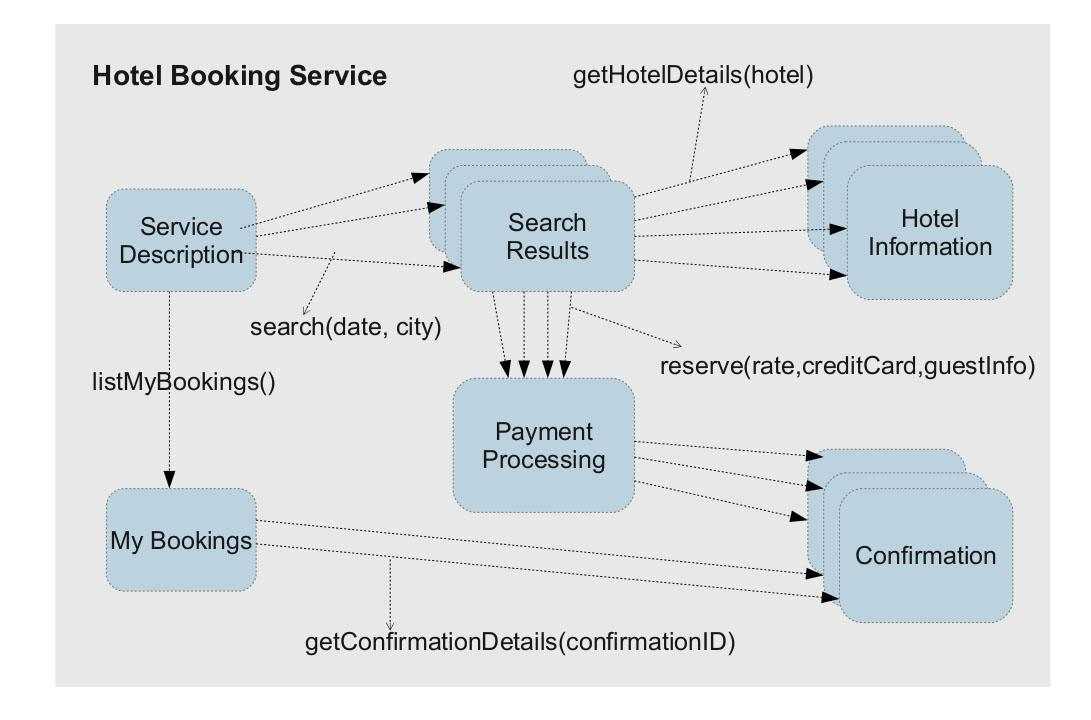
\includegraphics[scale=0.4]{images/hotel_booking.jpg}
        \caption{Structure of an Example Service}
        \label{fig:hotel_booking}
\end{figure}
The service description resource contains a form for searching for available hotels, given the number of guests, the start and end dates and the location. The search form serves as a link to search results resources, one per every unique combination of the input data — the form prescribes how to create a URI that contains the input data; the URI then identifies a resource with the search results. As there is a large number of possible search queries, there is also a large number of results resources, and the client does not need to know that all these resources are likely handled by a single program on the server. 

The search results are modeled as separate resources (as opposed to, for instance, a single data-handling resource that takes the inputs in an input message), because it simplifies the reuse of the hotel search functionality in other services or in mashups (lightweight compositions of Web applications), and it also enables caching of the results. With individual search results resources, creating the appropriate URI and retrieving the results (with HTTP GET) is easier in most programming frameworks than POSTing the input data in a structured data format to one Web resource, which would then reply with the search results. 
            
The service description also contains a link to a page with the bookings of the current user (which requires authentication functionality). With such a resource available to them, client applications no longer need to store the information about performed bookings locally.

Search results are a list of concrete rates available at the hotels in the given location, for the given dates and the number of guests. Each item of the list contains a link to further information about the hotel (e.g. the precise location, star rating and other descriptions), and a form for booking the rate, which takes as input the payment details (e.g. credit card information) and an identification of the guest who is going to stay in the room. The booking data is submitted (POSTed) to a payment resource, which processes the booking and redirects the client to a confirmation resource. The content of the confirmation can serve as a receipt.
             
Finally, the “my bookings” resource links to the confirmations of the bookings done by the authenticated user. The confirmations may further provide a way of canceling the reservation (not shown in the picture). 
           
Together, all these resources form the hotel booking service. However, the involved Web technologies actually work on the level of resources, so service is a virtual term here and the figure shows the service in a dashed box. 
        
So far, the description of the example hotel reservation service has focused on the hypermedia aspect: we described the resources and how they link to each other. Alternatively, and in fact more commonly, we can also view the service as a set of operations available to the clients — as an API. The search form in the homepage represents a search operation, the hotel information pages linked from the search results can be viewed as an operation for retrieving hotel details, the reservation form for any particular available rate becomes a reservation operation, and so on. 
          
While the resources of a service (the nouns) form the hypermedia graph (shown in Fig. 3.1), a programmer making a mashup or an automated client program rather thinks of the operations that can be invoked; therefore public RESTful Web services are generally called APIs and are described in terms of the operations. The following might be a typical operation description: 

The operation \texttt{getHotelDetails()} is invoked using the method GET at \\
\texttt{http://example.com/h/\{id\}}, with the ID of the particular hotel replacing the parameter id. It returns the hotel details in an ex:hotelInformation document.
\end{spacing}
\chapter{DESIGN}
\begin{spacing}{1.5}
This new solution uses a combination of Microformats-style markup and RDFS to provide a comprehensive framework for describing, discovering and composing RESTful services by adding semantics. Microformats, being simple and reusing a lot of the properties of HTML, provides users with a low entry-barrier for developers, which can increase adoption rate. These annotations are not visible to user but hidden in the HTML source and hence do not come in the way of users browsing the site.

In order to enable strong interlinking between services, a more robust solution like RDF and a backing RDF Schema is needed. This is achieved by providing an adapter for automatic conversion from the Microformat to RDF and providing a ready-made RDF Schema for the purpose(Figure: \ref{fig:micro_vs_rdf}). This way, the developers need not be concerned with the RDF descriptions that work in the background.

The solution currently addresses RESTful services that represent resources using JavaScript Object Notation (JSON). It is possible to extend the idea to XML based services as well by making some assumptions about the XML serialization.

\begin{figure}
        \centering
        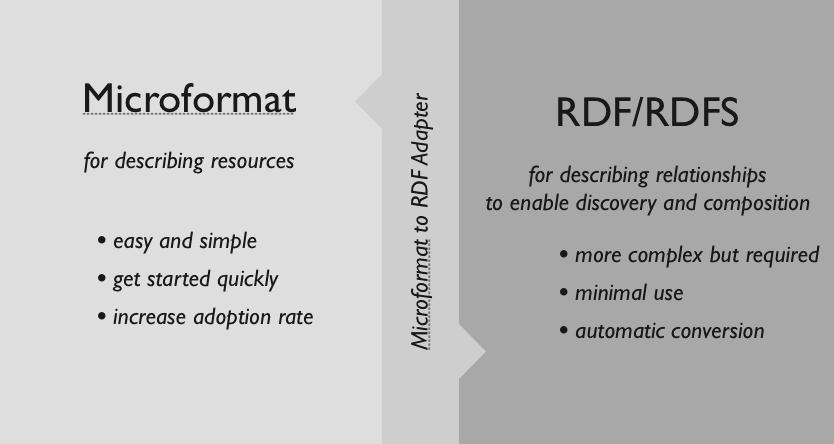
\includegraphics[scale=0.3]{images/micro_vs_rdf.png}
        \caption{Overview of the new architecture }
        \label{fig:micro_vs_rdf}
\end{figure}


\section{Service Description}

Services are described using special purpose annotations in the HTML code. These annotations are specified in the class attribute of the associated tags. This attribute is usually used for classification of HTML elements and also as selectors for JavaScript access and to style elements via CSS. Using special purpose annotations as class names help us to reuse whatever is already provided by HTML and JavaScript. Following annotations are proposed for describing resources in a RESTful API.

An intelligent agent extracts information about the service by traversing the DOM tree of the HTML page. APIs for traversing trees are available in almost all programming languages including JavaScript which is used extensively on the web and also to make extensions for many popular browsers such Chrome and Safari. Browsers or browser extensions could then could parse this data and automate the creation of clients for these services.


\section{Annotations}

Services are described using special purpose annotations in the HTML code. These annotations are specified in the class attribute of the associated tags.

\subsection{General Annotations}
\begin{enumerate}

\item {\bf hresource}: This is the root annotation that marks the resource description. All other annotations are contained within an element marked with class="hresource". A client parsing a page could treat the presence of this annotation as an indication of the existence of a resource description on the page. Unless all other annotations are encapsulated in an hresource, they will not be parsed.

\item {\bf name} :Annotates the name of the resource. This can be any human readable name and need not have any programming significance.

\item {\bf url/uri}: Annotates the URL at which the resource is accessible.
\end{enumerate}

\subsection{Annotation of Methods}
Annotates Permissiable methods (GET,POST,PUT,DELETE)

\begin{enumerate}
\item {\bf method}: This is the root annotation that marks the permissiable method. It contains following sub-annotations
\begin{itemize}
\item {\it type}: HTTP request type. GET,POST,PUT,DELETE
\item {\it input}:  (optional) input attribute
\item {\it output}: (optional) output attribute
\item {\it header}: (optional) attributes that should be passed as header to HTTP request
\end{itemize}
\end{enumerate}

\subsection{Annotation Of Attributes}
\begin{enumerate}
\item {\bf attribute}: Annotates an attribute/property of the resource. All attributes of a resource should be annotated with this annotation. Specific characteristics of the attribute could be further specified by more annotations that are used together with the attribute annotation.

\item {\bf required}: Indicates a required attribute. This annotation is always used along with the attribute annotation.

\item {\bf queryable}:  Indicates an attribute that may be provided in the HTTP querystring during a GET operation to filter the results. This annotation is always used along with the attribute annotation.

\item {\bf read-only}:  Indicates a read-only attribute. A read-only attribute may be retrieved during a GET operation but may not be included in a POST or a PUT. This annotation is always used along with the attribute annotation.write-once: Indicates a write-once attribute that can be specified only during the create operation (POST) but not during update (PUT). This annotation is always used along with the attribute annotation.

\item {\bf guid}: Indicates if an attribute is a globally unique identifier for the resource that could be used across multiple services.
\item {\bf Comment}: Provides a human-readable description of the attribute. This should be descendant of parent of attribute node

\item {\bf hresource-datatype}: Annotates the datatype of the attribute.This should be descendant of parent of attribute node.For permissible types see table: \ref{tab:data_types}

\begin{table}
    \centering
    \begin{tabular}{|l|l|}
    \hline
    Data Type      & Description                    \\ \hline
    Integer or Int &  32 bit integer                \\ \hline
    float          & floating point number          \\ \hline
    Int64          &  64 bit integer.               \\ \hline
     Range         &  Boolean or Bool               \\ \hline
    Date or Time   & should specify date formatting \\ \hline
    Timestamp      & Timestamp of entity            \\ \hline
    \end{tabular}
    \caption{Data types}
    \label{tab:data_types}
\end{table}

{\bf eg}: Range(0.0,1.0) specifies floating point number between 0 and 1 and Range(0,1) specifies integer between 0 and 1.
\end{enumerate}

\subsection{Annotation of Errors}

\begin{enumerate}
\item {\bf hresource-error}: This is the root annotation that marks the errors.It should contain two sub-annotation for each error:
\begin{itemize}
\item {\it error-code}:Specify the error code.
\item {\it comment}: Description of error.
\end{itemize}
\end{enumerate}
eg:
\begin{minted}{html}
<li class="hresource-error">
      <code class="error-code">201$</code>-<span class="comment">
      test failed</span>
      </li>
\end{minted}

The relationship between these sematnic annotataion is shown in figuere \ref{fig:rel_semantic} (hresource-produced-by and hresource-consumed-by are described in section \ref{sec:service_disc})
\begin{figure}
        \centering
        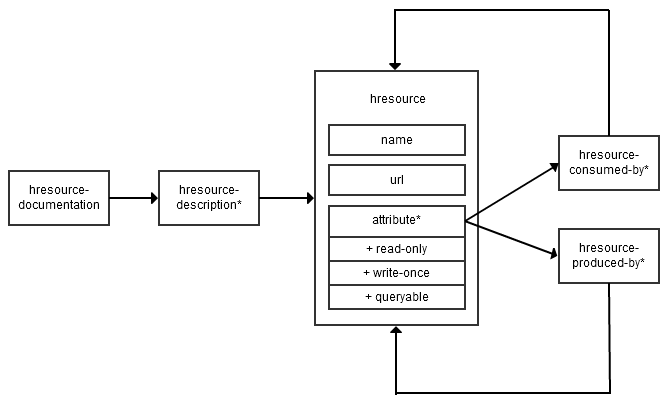
\includegraphics[scale=0.5]{images/rel_semantic.png}
        \caption{Relationship between the semantic annotations}
 ('*' indicates a one-to- many relationship)
        \label{fig:rel_semantic}
\end{figure}


An intelligent agent extracts information about the service by traversing the DOM tree of the HTML page(See figure \ref{fig:code}. APIs for traversing trees are available in almost all programming languages including JavaScript which is used extensively on the web and also to make extensions for many popular browsers such Chrome and Safari. Browsers or browser extensions could then could parse this data and automate the creation of clients for these services.

%include code.
\begin{figure}
\begin{minted}{html}

<div class="hresource">
  <h1 class="name">User</h1>
  URL:
  <span class="url">
    http://example.com/api/user
  </span>
  <p class="comment">
    api desc(Human Readable) - It is a <a rel="hresource-is-a"

    href="http://dublincore.org/user/">user</a>
  </p>
  <div class="method">
      It use HTTP <span class="type">GET</span> request with:<br>
      Inputs:
      <ul>
          <li class="input">username</li>
          <li class="input">password</li>
          <li class="input">country</li>
      </ul>
      Produces:
      <ul>
          <li class="output">userid</li>
      </ul>
  </div>
  <ol>
    <li>
      <code class="attribute required write-once queryable">
        username
      </code> -<span class="comment">
      username -required, must be unique.</span>
    </li>
    <li>
    \end{minted}
\caption{Description for a User resource in an annotated web page -Part 1}
\label{fig:code}
\end{figure}
\begin{figure}
    \begin{minted}{html}
      <code class="attribute required">
        password
      </code> -<span class="comment"> required.</span>
    </li>
    <li>
      <code class="attribute queryable">
      country</code>(<span class="hresource-datatype">string</span>)
      <div>
        Producers:
        <ul>
          <li><a rel="hresource-produced-by"
          href="http://xyz.com/cn#country">cn</a></li>
          <li><a rel="hresource-produced-by"
          href="http://abc.com/getcountry#country">
          getcountry</a></li>
        </ul>
      </div>
    </li>
    <li>
      <code class="attribute read-only">
       userid
      </code>-<span class="comment">userID returned as result</span>
    </li>
  </ol>
  <p>ERRORCODE</p>
\end{minted}

\begin{minted}{html}
  <ol>
    <li class="hresource-error">
      <code class="error-code">550</code> -<span class="comment">
      no such user</span>
  </ol>
</div>
\end{minted}
\caption{Description for a User resource in an annotated web page. - Part 2}
\label{fig:code2}
\end{figure}

\section{Service Discovery}
\label{sec:service_disc}

The discovery mechanism works to enable discovery of new, similar and related services. Service discovery addresses two different aspects of the problem: discovery by users and discovery by services.
\begin{enumerate}
\item {\it Discover-as-you-browse}: This deals with enabling browsers (or browser extensions) to hint users about the presence of resources as they browse a website. This works similar to how users discover RSS feeds(Figure \ref{fig:rss_api}). link element provided by HTML is used to alert browsers about the presence of REST resources on the website. This can be supplemented with automatic client creation since the browser can now link to the resource descriptions and read the data from the page using DOM traversal. The syntax of the link tag to use is as follows:

\begin{minted}{html}
<link rel="hresource-documentation"
    href="http://example.com/api/" />
\end{minted}


The tag goes into the header of a page and the value hresource-documentation in the rel attribute specifies that the linked item is a REST resource. From the documentation page, links to individual resources in the API are annotated with hresource-description as the value of the rel attribute:

\begin{minted}{html}
<a rel="hresource-description"
        href="http://example.com/api/user/">User</a>
\end{minted}

The annotation is added to each resource linked from the API documentation start page. The client thus traverses from the homepage to the documentation page and from there to the individual resource descriptions to discover the resources and present this to the user.

\item {\it Automated Discovery}: Automated discovery deals with the ability of a service to discover similar services in the same domain and to link to them. Service discovery allows clients to find services that could provide data required to access another service or could consume data received from another service. Existing service discovery mechanisms use a directory-oriented approach and are suited only for SOAP based services. The new description syntax provides a discovery mechanism for RESTful services that works peer-to-peer without any dependence on a central controller.

The system works by identifying the different links as it comes across new resources and building up a graph connecting them. At a later stage, this graph could be traversed to discover new possibilities and to look for other sources of input.
\end{enumerate}

\begin{figure}
        \centering
        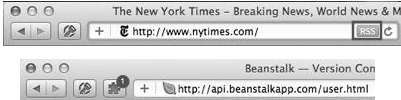
\includegraphics[scale=0.8]{images/rss_api.png}
        \caption{ The RSS discovery mechanism already present in modern browsers.}
        The toolbar button shows a badge with the number of resources found when visiting a site with embedded resource descriptions.
        \label{fig:rss_api}
\end{figure}

The following annotations for inter-links between services are defined to enable discovery:

\begin{enumerate}
\item {\it Link to Superclass}: When a resource is a subclass of another resource, this link is indicated by the rel attribute hresource-is-a. This implies that wherever the superclass is accepted, the subclass is also accepted. For e.g., if a publisher defines a Book resource to provide a search of their catalog, they could annotate the resource to be a subclass of a more generic Book resource.

\begin{minted}{html}
<a rel="hresource-is-a"
               href="http://dublincore.org/book/">
               Book
        </a>
\end{minted}

If there is another service from a bookshop that is known to accept a generic book resource for a purchase process, the client could infer that the specific book resource from the catalog would also be accepted there and use it.

For this linking to work properly, we need a core set of resources that can be extended by others. Fortunately, there is already a project named Dublin Core running that has defined many commonly used resources. We could reuse these resources for our purpose and use them as the root resources.

\item {\it Link to Consumers}: When an attribute of a service is consumed by another known service, this is annotated using \texttt{a rel attribute hresource-consumed-by}. This enables a software agent to find out what all can be done with the resource that it has already retrieved.

\begin{minted}{html}
<code class="attribute">
             ISBN
        </code>
        Consumers:
        <ul>
            <li rel="hresource-consumed-by">
               http://bookshop.com/book-order\#isbn
            </li>
            <li rel="hresource-consumed-by">
               http://library.com/rented-book\#isbn
            </li>
        </ul>
\end{minted}

\item {\it Link to Producers}: Similar to the link to consumers, services can annotate a link to a producer of one of its attributes. This helps reverse traversal of resources and also makes the system more peer-to-peer. This way, a link needs to be provided in either at one of the consumers or at the provider and an agent can identify this with link traversal. The annotation is made with the rel attribute \texttt{hresource-produced-by}.

\begin{figure}
        \centering
        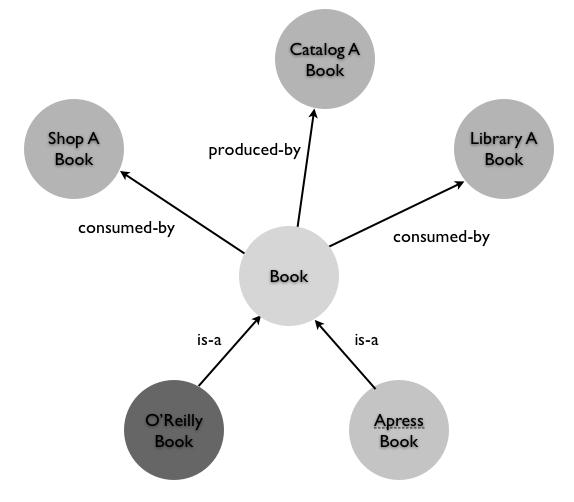
\includegraphics[scale=0.5]{images/res_graph.png}
        \caption{A graph constructed from the links between the resources.}
        \label{fig:res_graph}
\end{figure}

\section{Composition}

Service composition is made possible by using the same annotations that were made for discovery. A graph is constructed starting from a resource and then traversing the parent, consumer and producer links recursively. At each page, the descriptions are extracted and converted to RDF to update the graph. This way, a software agent that does not have the identifier or a search parameter to access a specific resource could traverse the graph to figure out what other information could be used to lookup the identifier and present the choice to the user.

For e.g., the service provided by a bookshop might need the ISBN to order a book. However, the traversal of the graph could reveal a catalog service that retrieves book resources using titles or author names. This allows the software agent to provide a choice to the user where he can enter either the ISBN or the title.

This works in the reverse direction also. Having received access to a resource, the software agent can suggest what all operations can accept the resource. So effectively a service that has a book resource can provide options for services from shops that let the user order the book or libraries that let the user lend the book .
\end{spacing}
\chapter{IMPLEMENTATION}
\begin{spacing}{1.5}
The proposed system currently addresses the composition of RESTful web services that represent resources using the JavaScript Object Notation (JSON). The system expexts the services to return results to API queries as JSON objects and composes them as per the user specification. Extension of the same idea can enable the composition of XML based RESTful services.The system also includes an RDF conversion module that performs the automatic conversion process from Microformat annotations to RDF.

The system uses a web UI developed in HTML, JavaScript as the frontend for reading user input. The requests are handled by a server program developed in node.js that accepts requests from multiple client machines and handles them asynchronously. The server program acts as a proxy and is developed to enable the system to handle high volumes of client traffic. The server does the bulk of orocessing and also allows multiple cross domain HTTP calls with ease, which would otherwise be not possible with a client side implementation because of the same origin policy enforced by the modern web browsers. The basic architecture of the system is as illustratred in Figure: \ref{fig:architecture}

\begin{figure}
        \centering
        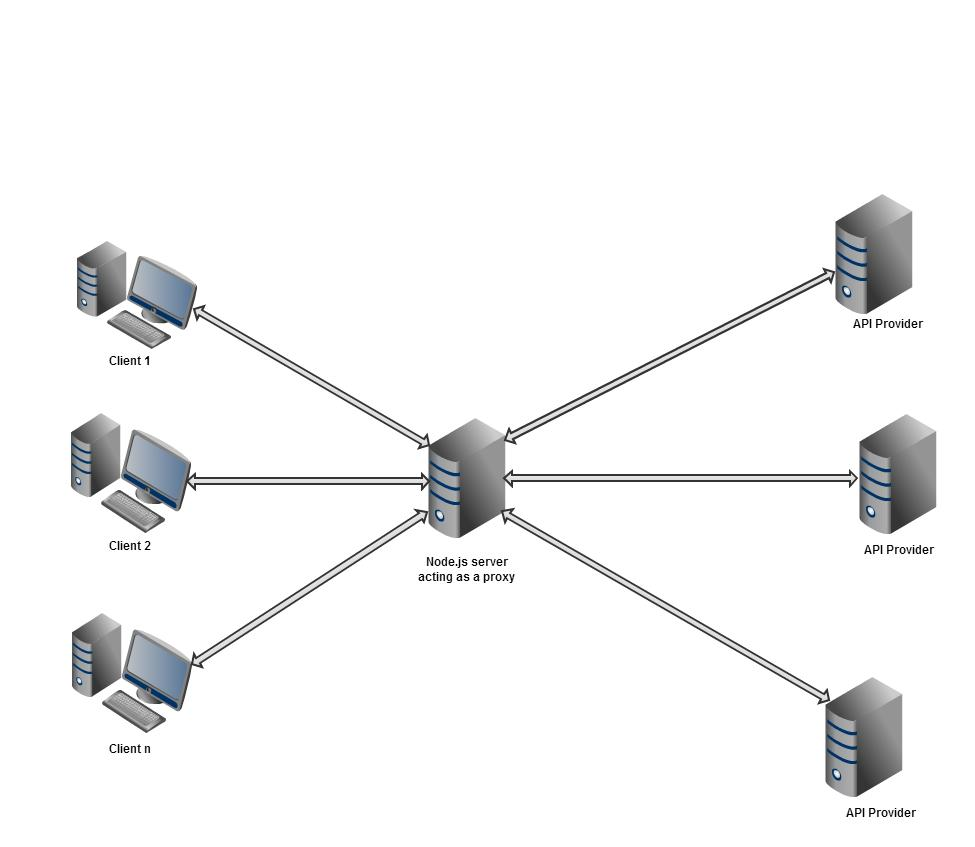
\includegraphics[scale=0.3]{images/Architecture.jpg}
        \caption{System architecture }
        \label{fig:architecture}
\end{figure}

The system uses a parser module to parse the DOM tree of the annotated API Documentation page and extract the information embedded in it. Based on users input of which APIs to use for composition, the server fetches each of the required annotated API documentation pages and parses them. Based on the information extracted from DOM tree, the web UI presented to the user is populated with a set of API operations that the system identifies and that can be composed. A workbench is presented to the user and a drag-drop based user interface enables the him/her to graphically descipbe the required composition of web services. Once the mashup is graphical design of the mashup is complete and user submits it, information from the design is converted into an abstract internal representation that is passed to the server. The server now invokes the reqired API calls asynchronouly and composes them as required and produces an HTML formatted output which is the required mashup. The HTML output is then served back to the client system for the user. The interaction flow in the system is illustrated in Figure: \ref{fig:sequence}

\begin{figure}
        \centering
        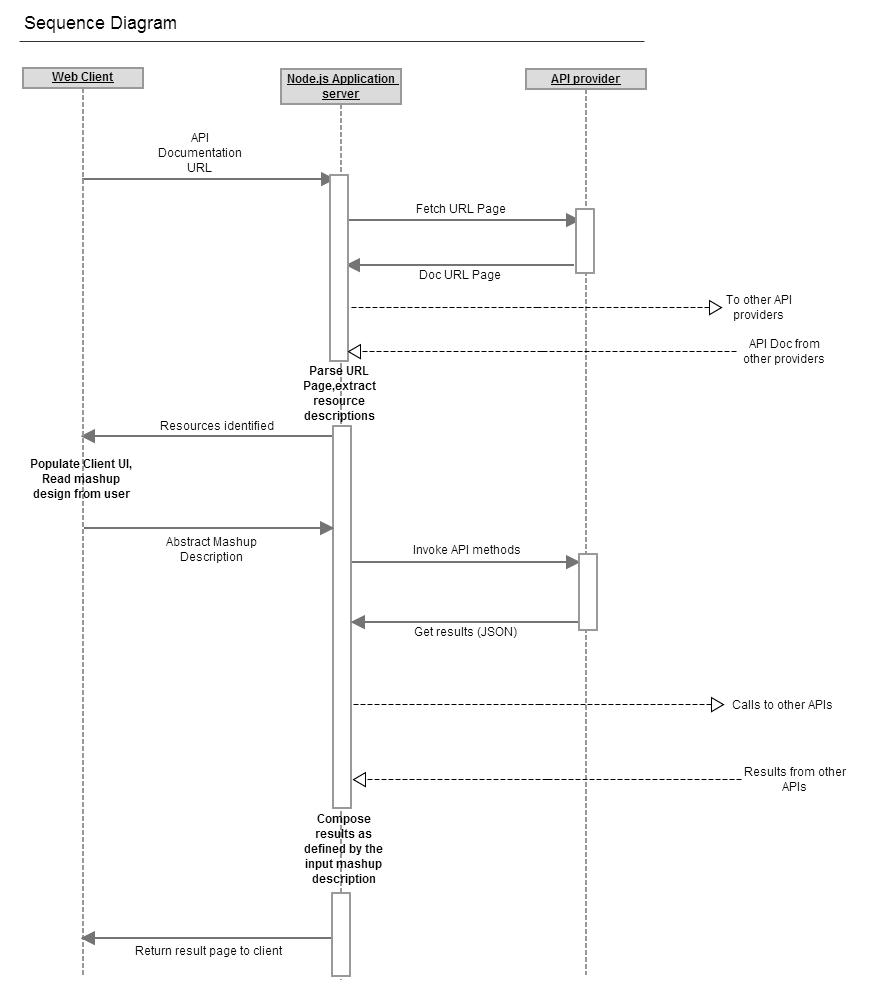
\includegraphics[scale=0.5]{images/smashup_sequence.jpg}
        \caption{Interaction flow sequence}
        \label{fig:sequence}
\end{figure}

\section{Server side Implementation}
The architecture of the server is as illustrated in Figure: \ref{fig:serverarch}.Server primarily deals with providing three services:
\begin{enumerate}

\item{\bf Parsing API Documentation HTML}: Client side provides a URL to an annotated API Documentation HTML page. The server fetches the required documentation page and passes the HTML DOM to the parser module {\it(hrestsparser)}. The parser generates a JSON description of the annotated resources which is then passed to the client to populate the client UI. The parser uses XPath for the traversal of the DOM tree and hence platform neutral.

\begin{figure}
        \centering
        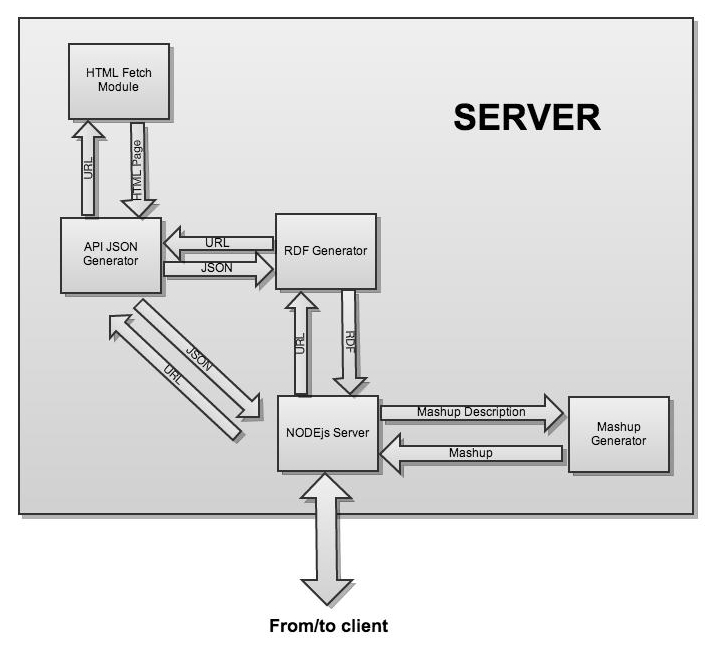
\includegraphics[scale=0.4]{images/Server_Architecture.jpg}
        \caption{Server Architecture}
        \label{fig:serverarch}
\end{figure}

\item{\bf RDF Generation}: Client passes a URL to the server. The page is fetched by the RDF generator module. The page is parsed by the hRESTS parser module to produce the output JSON. The {\it produced-by} - {\it consumed-by} relations in the annotated page forms a graph of resources each of which is required for the generation of the RDF description. The RDF generator module recursively traverses the producer-consumer graph and fetches each of the required resources upto some arbitrary level of nesting. Once the resource fetching is done RDF can be generated.

\item{\bf Request handling and mashup generation}: The user specifeis the required composition of services graphically in the client workbench. An abstract description of the required mashup is generated at the client and is passed to the server as a JSON object. The server makes the required API invocations to fetch each of the resources to be composed into the final mashup. The description JSON is parsed and the result resources are composed as specified producing an HTML output which is then served to the client system.
\end{enumerate}

\section{Client side Implementation}
Client provides a simple drag and drop based user interface for mashup design. The elements in the UI are populated from the contents of the API documantations passed to the server. The different API calls can be simply dragged and dropped to the workbench and the inputs and outputs can be piped to one another by graphical connectors.

Client uses two basic data structures which are simple JSON objects.
\begin{itemize}
\item{\bf docjsons}: An array of JSON description of all APIs loaded into the workbench
\item{\bf attributearray}: An associative array indexed using the ID of the API call used ( one for each widget used in the workbench). It has the following components:
\begin{enumerate}
\item{\it jindex}: Index of document JSON in array of JSONs.
\item{\it apiindex}: Index of the particular API used in this JSON
\item{\it isStartNode}: True if there are no inputs piped into this node ,i.e, this node is a start point in the mashup design with inputs from the user and not from other API calls.
\item{\it method}: HTTP method selected by the user.
\item{\it inputs}: An associative array of inputs indexed by attribute name.
\item{\it outputs}: An associative array of outputs indexed by attribute name.
\item{\it headers}: An associative array containing the headers to be passed (if required) with an API call, indexed by attribute name.
\end{enumerate}

Each element in the inputs array has two attributes :
\begin{itemize}
\item{\it value}: Value of the attribute or null.
\item{\it link}: Null or a tuple (id of the producer API call,name of the attribute producing it)
\end{itemize}

Each element in the outputs array has a single attribute:
\begin{itemize}
\item{\it link}: Null or a tuple (id of the consumer API call,name of the attribute that consumes it)
\end{itemize}

\end{itemize}

The link attributes forms a logical graph of the way in which the different service calls are composed. An abstract representation of the mashup is created by traversing the graph. The traversal is done by using a simple modification to the Depth First Search technique. The abstract representation is a JSON object which represents the initiation sequence for the API calls. This is then passed to the server.

\section{Tools and Technologies}

\subsection{Resource Description Framework (RDF)}
RDF is a W3C standard\cite{rdf} for modeling and sharing distributed knowledge based on a decentralized open-world assumption. Any knowledge about anything can be decomposed into triples (3-tuples) consisting of subject, predicate, and object; essentially, RDF is the lowest common denominator for exchanging data between systems.RDF is designed to be read and understood by machines.It is normally written in XML.RDF is a part of W3C's semantic web activity.

What makes RDF suited for distributed knowledge is that RDF applications can put together RDF files posted by different people around the Internet and easily learn from them new things that no single document asserted. It does this in two ways, first by linking documents together by the common vocabularies they use, and second by allowing any document to use any vocabulary. This flexibility is fairly unique to RDF.

The use cases of RDF, as described by Richard Cyganiak on the W3C's Semantic Web activiy is as follows:
\begin{itemize}
\item{to integrate data from different sources without custom programming.}
\item{to offer your data for re-use by other parties.}
\item{to decentralize data in a way that no single party {\it owns} all the data.}
\end{itemize}


RDF describes resources as tripples with subject as the identifier of the resource,predicate as the property and object as the value of the property.The linking structure of RDF forms a directed, labeled graph, where the edges  represent the named link between two resources, represented by the graph nodes.This graph view is the easiest possible mental model for RDF and is often used in easy-to-understand visual explanations.


\subsection{Bootstrap Framework}
Bootstrap is a front-end toolkit developed by twitter for rapidly developing web applications\cite{bootstrap}.It contains HTML and CSS-based design templates
for typography, forms, buttons, charts, navigation and other interface components, as well as optional JavaScript extensions. At its core, Bootstrap is just CSS, but it's built with Less, a flexible pre-processor that offers much more power and flexibility than regular CSS. With Less, it gains a range of features like nested declarations, variables, mixins, operations, and color functions. Additionally, since Bootstrap is purely CSS when compiled via Less, two important benefits are observed:

First, Bootstrap remains very easy to implement; just drop it in your code and go. Compiling Less can be accomplished via Javascript, an unofficial Mac application, or via Node.js.

Second, once complied, Bootstrap contains nothing but CSS, meaning there are no superfluous images, Flash, or Javascript.All that remains is simple and powerful CSS for your web development needs.

We used bootstrap for cross browser compatibility.The front end of the client side is built on top of bootstrap framework.

\subsection{JSPlumb}
jsPlumb provides a means for a developer to visually connect elements on their web pages.It uses Bezier curve functions for plotting connections in the user interface.jsPlumb can be used with jQuery, MooTools or YUI3 (or another library of your choice).It provides an API with many options like bind(Bind to an event on jsPlumb),connect(establish a connection between two elements),select(select a set of connections using filter option) etc.To connect between any two elements in the UI,the id of the source and target must be specified.

We used jsPlumb to visualize the creation of the mashups.When resource description embedded in a web page is parsed,the available resources are presented to the user.The user can then make connections between the resources to form mashups.Whenever a connection is specified by the user the input,output parameters to create mashups are collected from the user,and a client is generated automatically.

\subsection{Node.js}
Node.js is a platform built on Chrome's JavaScript runtime for easily building fast, scalable network applications. Node.js uses an event-driven, non-blocking I/O model that makes it lightweight and efficient, perfect for data-intensive real-time applications that run across distributed devices. It is a server-side system for writing scalable internet applications ,notably web servers.

Node.js contains a built-in HTTP  server library\cite{nodejs},making it possible to run a web server without the use of external software such as Apache or Lighttpd, and allowing more control of how the web server works. Node.js enables web developers to create an entire web application in JavaScript,both server-side and client-side. Node.js is very fast(event-loop non-blocking) and also has very speedy native bindings. Performance is the main advantage of Node.js; it allocates a small heap per each connection, while other server side solutions create a (2MB) thread for each incoming connection, and of course creating a thread is much slower than allocating heap memory. Also being written in JavaScript lowers the barrier to entry for most front-end developers who are already used to working with the language.

Node.js is used in this design to solve the problem of making cross domain calls. Apart from that, it provides good performance with large  no of services used to create mashups. We stick to Node.js with the  thought  that an event driven architecture can lead to more scalable applications. Also it is lightweight and  perfect for data-intensive real-time applications that run across distributed devices.


\end{spacing}


\chapter{OUTPUT}
\begin{spacing}{1.5}
The screenshots of the prototype program developed. The entire source code is available in GitHub - {\it https://github.com/abilng/sMash.it}

\begin{figure}
        \centering
        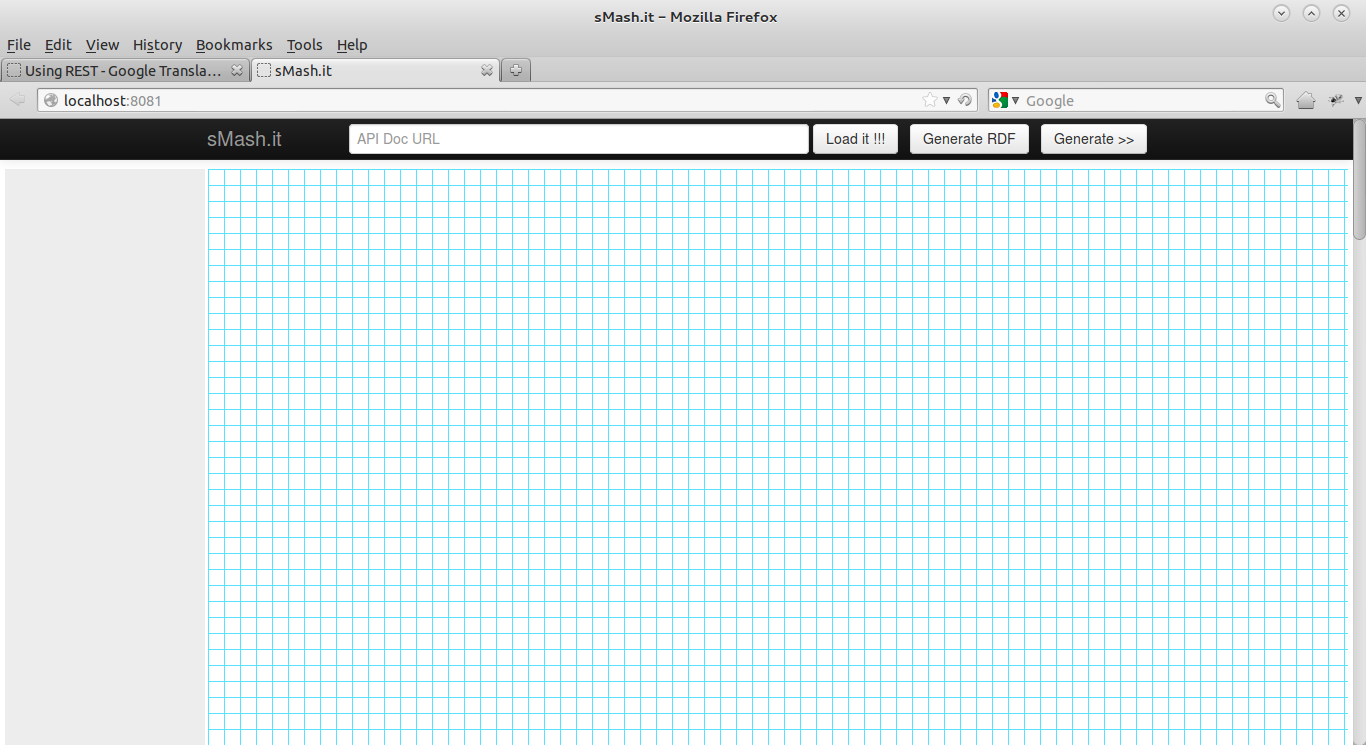
\includegraphics[scale=0.3]{images/7.png}
        \caption{Client Homescreen and workbench}
\end{figure}

\begin{figure}
        \centering
        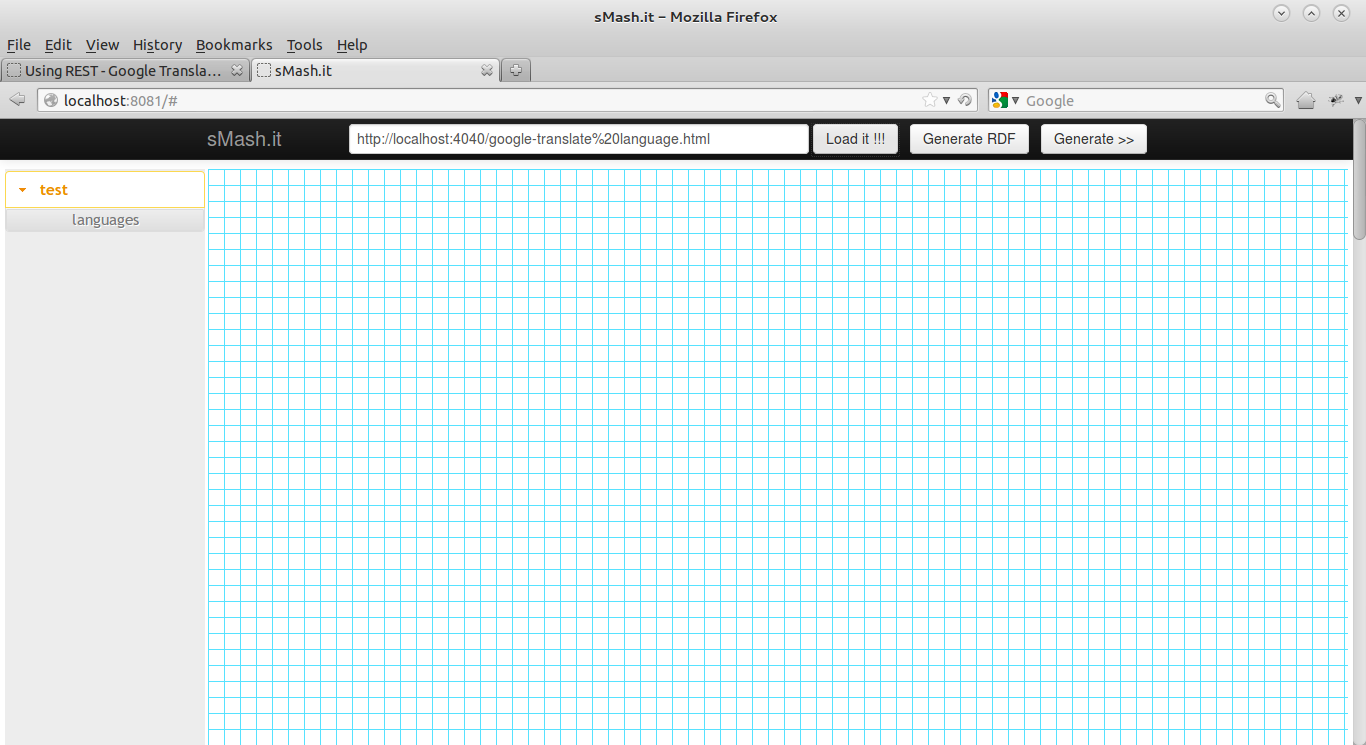
\includegraphics[scale=0.3]{images/6.png}
        \caption{Loading an API}
\end{figure}


\begin{figure}
        \centering
        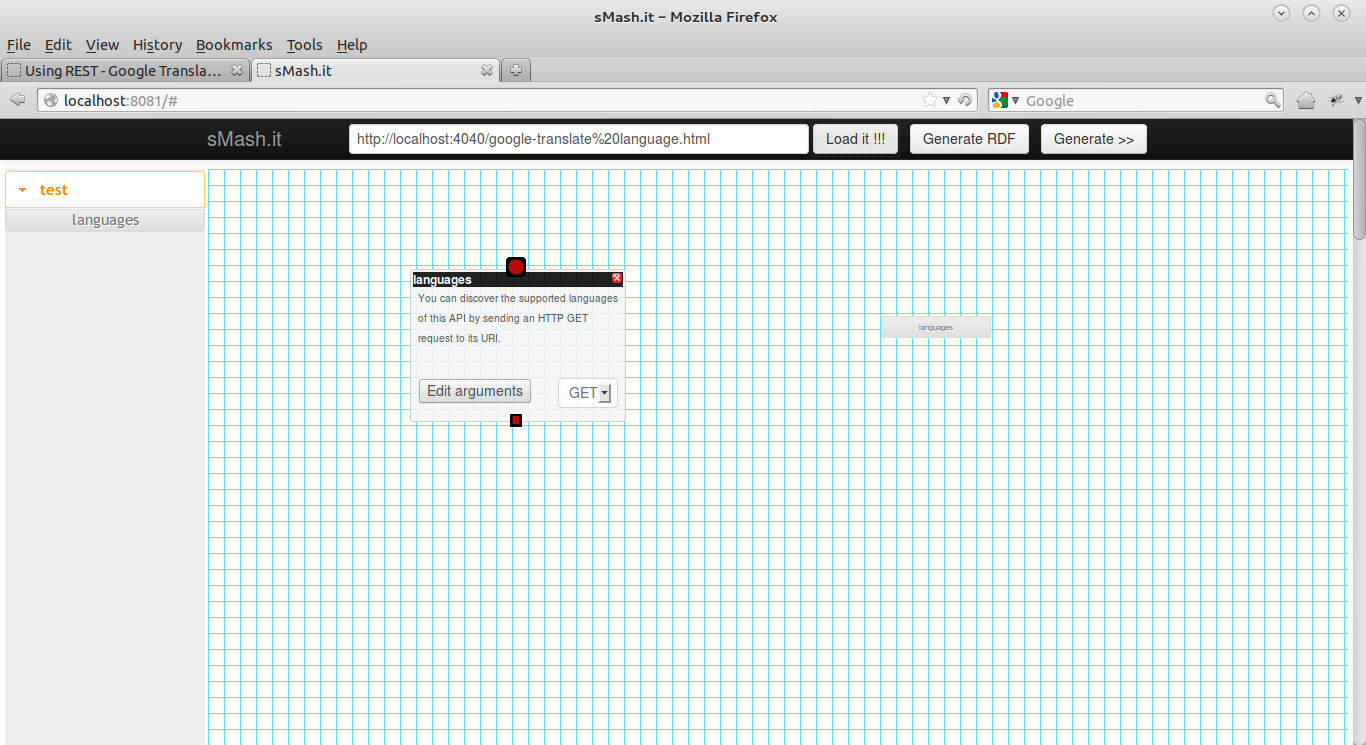
\includegraphics[scale=0.3]{images/5.png}
        \caption{Mashup design using drag n drop - step 1}
\end{figure}

\begin{figure}
        \centering
        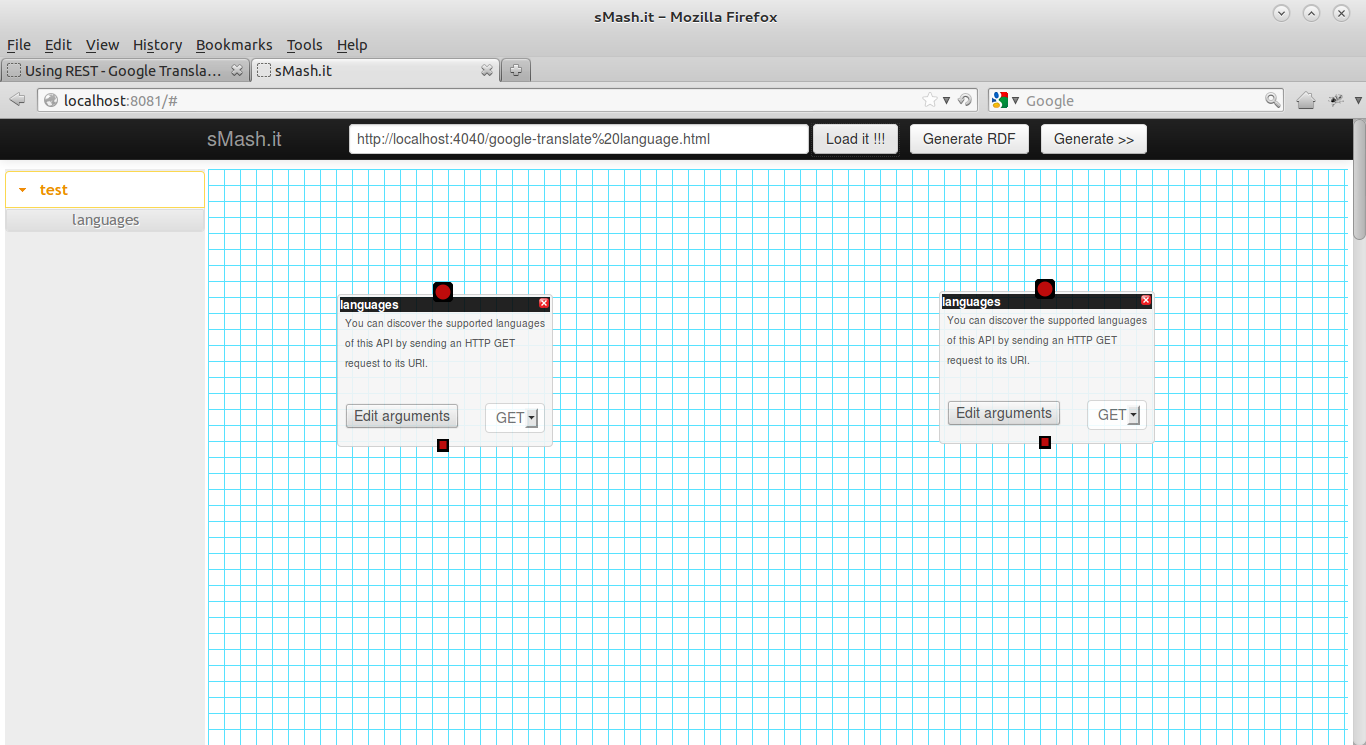
\includegraphics[scale=0.3]{images/4.png}
        \caption{Mashup design using drag n drop -step 2}
\end{figure}


\begin{figure}
        \centering
        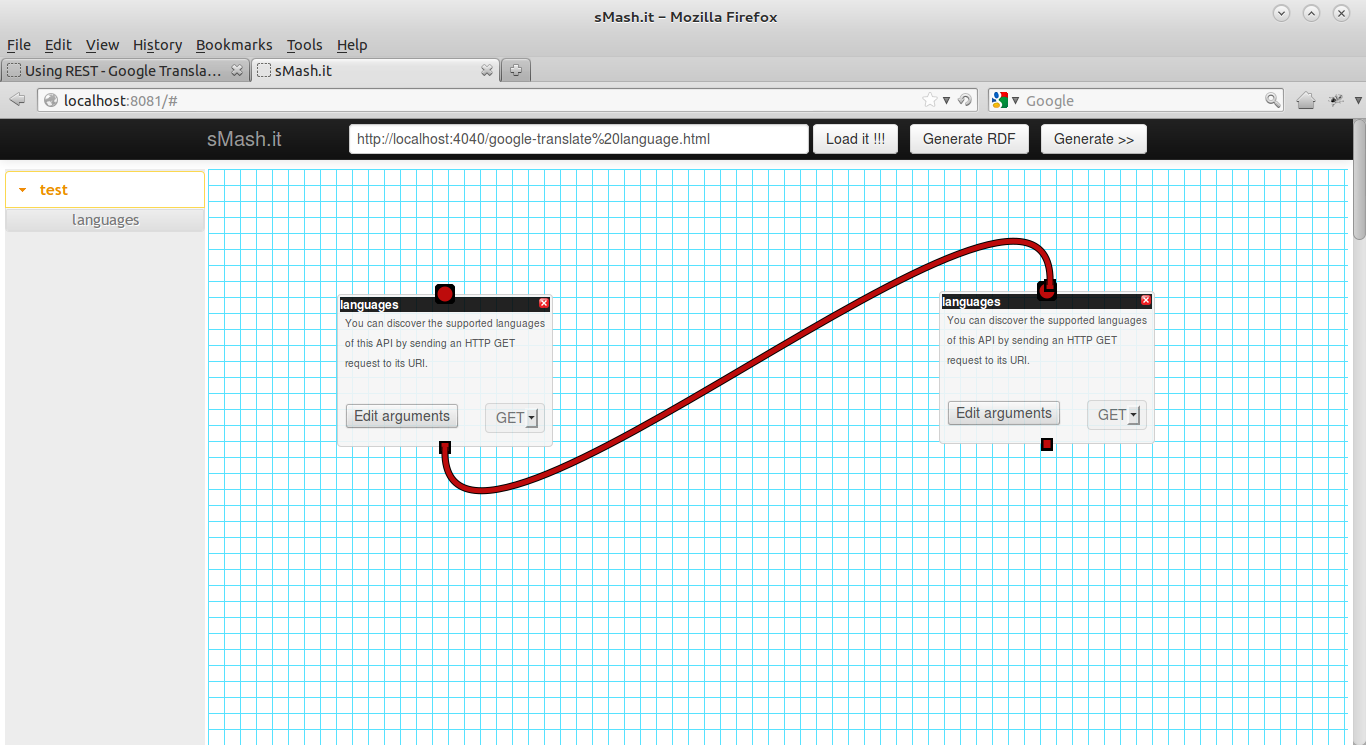
\includegraphics[scale=0.3]{images/3.png}
        \caption{Mashup design using drag n drop -step 3}
\end{figure}


\begin{figure}
        \centering
        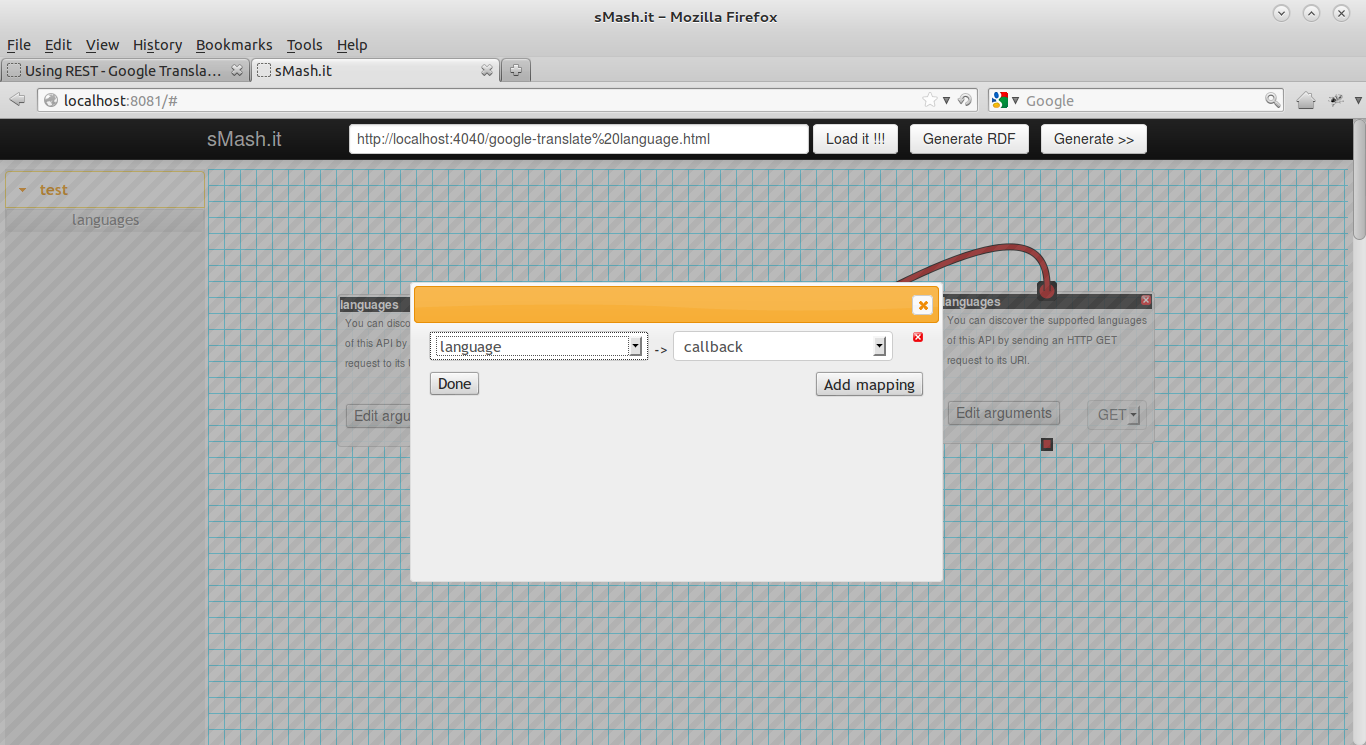
\includegraphics[scale=0.3]{images/2.png}
        \caption{Mashup creation-step 4, Parameter mapping.}
\end{figure}

\begin{figure}
        \centering
        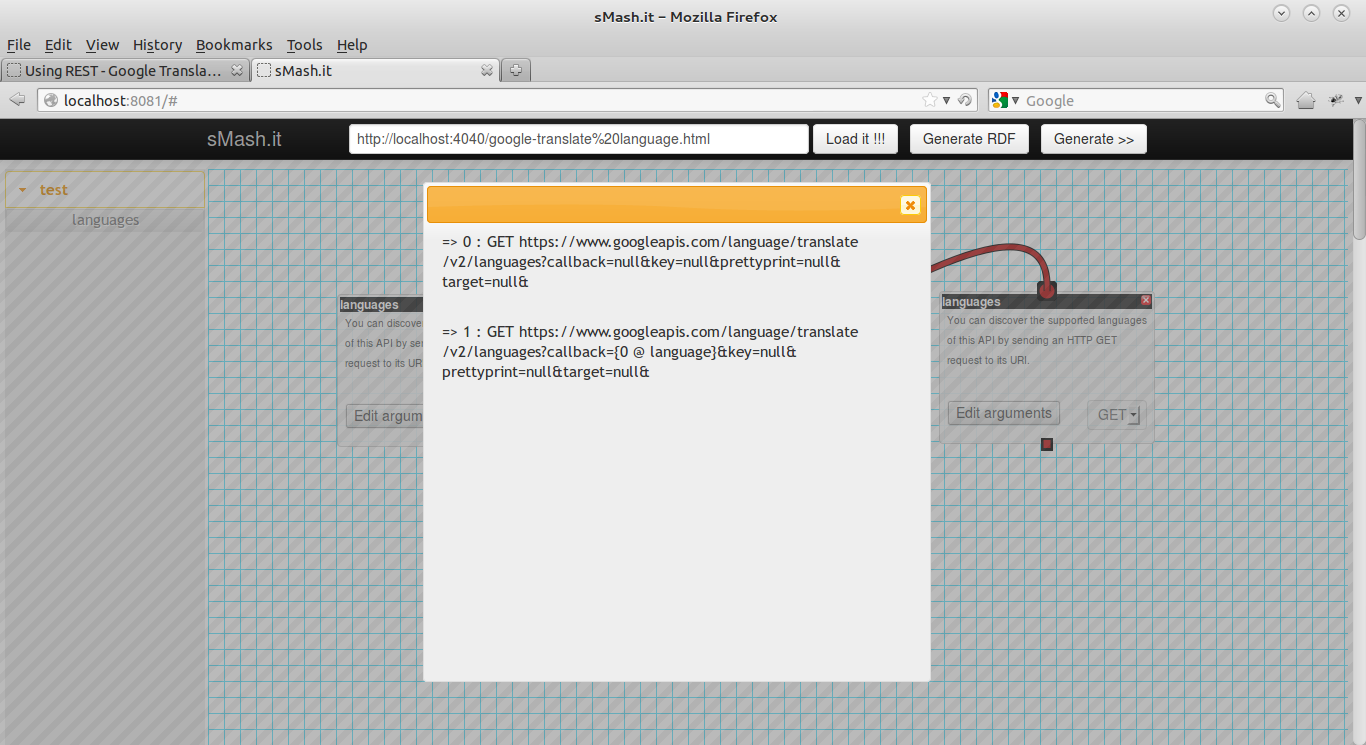
\includegraphics[scale=0.3]{images/1.png}
        \caption{Invocation sequence generated.}
\end{figure}
\end{spacing}
\chapter{Conclusion}
\begin{spacing}{1.5}
Web is increasingly getting complex these days. Thousands of services spwan millions of requests each day. This work envisioned a intelligent web framework in which a service can create interconnections between diffrents services compatible. It opens up a multitude of possibilities, including a higher layer maniputation of information for what it represents than how it is represented.

Popularisation of services like ifttt have given us the proof that this service is inevitable in the future of web, and if machines were able to parse the information constituded by entire internet it can do wonders that no one envisioned, so it can only be comapred with magic.

The prototype mashup editor created can intelligintly mash the services based on annotoations But it is also limited in some aspects. But we hope this  direction deserves more exploration since it is relativly easy for the developer and the machine to follow. The prototype was implimented in different paradigms to verify the computatuiional completetability.

The imeediate future directions we would like to purse this works are
\begin{enumerate}
\item Change to accomodate todays REST APIs. Most of the rest apis in use today does to conform to the RESTful paradigm. They uses GET heavily to get most of the things done for perfomance purposes. This have to taken care of.

\item A tool to convert exishting REST APIs.
But this comes with lot of challenge. The above one for a start, adoption is another problem.
\end{enumerate}
\end{spacing}


\begin{thebibliography}{9}

\bibitem{1}
	1. Christian Bizer, Tom Heath, Tim Berners-Lee,
	\emph{1. Linked Data - The Story So Far}.
	in International Journal on Semantic Web and Information Systems IJSWIS, 2009..
\bibitem{2}
	Frank Manola, Eric Miller, Brian McBride,
	\emph{“RDF Primer”},
	W3C Recommendation, 10 February 2004.

\bibitem{3}
	Dborah L. McGuinness, Frank van Harmelen,
	\emph{“OWL Web Ontology Language: 	Overview”},
	W3C Recommendation, 10 February 2004.
\bibitem{4}
	W3C OWL Working Group,
	\emph{“OWL 2 Web Ontology Language: Document Overview”},
	W3C Recommendation, 27 October 2009.
\bibitem{5}
	Dan Brickley, R.V. Guha, Brian McBride,
	\emph{“RDF Vocabulary Description Language 1.0: 	RDF Schema”},
	W3C Recommendation, 10 February 2004.
\bibitem{6}
	Microformats -
	\emph{http://www.microformats.org/.}
\bibitem{7}
	Ben Adida, Mark Birbeck, Shane McCarron, Steven Pemberton,
	\emph{“RDFa in XHTML: 	Syntax and Processing: A collection of attributes and processing rules for extending 	XHTML to support RDF”},
	W3C Recommendation, 14 October 2008.
\bibitem{8}
	Ben Adida, Mark Birbeck,
	\emph{“RDFa Primer - Bridging the Human and Data Webs”},
	W3C 	Recommendation, 14 October 2008.
\bibitem{9}
	R.T. Fielding,
	\emph{“Architectural styles and the design of network-based software       	architectures”},
	PhD dissertation, Department of Information and Computer Science, 	University of California, Irvine, 2000.
\bibitem{10}
	Roberto Chinnici,Jean-Jacques Moreau, Arthur Ryman, Sanjiva Weerawarana,
	\emph{“Web 	Services Description Language (WSDL) Version 2.0 Part 1: Core Language”},
	W3C 	Recommendation, 26 June 2007.
\bibitem{11}
	Marc Hadley,
	\emph{“Web Application Description Language”},
	W3C Member Submission, 31 	August 2009.
\bibitem{12}
	Jacek Kopecky, Karthik Gomadam, Tomas Vitvar,
	\emph{“hRESTS: an HTML Microformat for 	Describing RESTful Web Services,”} IEEE/WIC/ACM International Conference on Web 	Intelligence and Intelligent Agent Technology, 2008.
\bibitem{13}
	Karthik Gomadam, Ajith Ranabahu, Amit Sheth,
	\emph{“SA-REST: Semantic Annotation of 	Web Resources”},
	W3C Member Submission, 05 April 2010.
\bibitem{14}
	Markus Lanthaler, Christian Gütl,
	\emph{“A Semantic Description Language for RESTful Data 	Services to Combat Semaphobia”},
	5th IEEE International Conference on Digital 	Ecosystems and Technologies (IEEE DEST 2011), 31 May -3 June 2011, Daejeon, Korea.
\bibitem{15}
	Douglas Crockford,
	\emph{“RFC 4627: The application/json Media Type for JavaScript Object 	Notation (JSON)”},
	Network Working Group, July 2006.
\bibitem{jsplumb}
	jsPlumb documentation -
	\emph{http://jsplumbtoolkit.com/doc/home.html}
\bibitem{api}
	API Documentation -
	\emph{http://jsplumbtoolkit.com/apidocs/files/jsPlumb-1.4.1-apidoc.html}
\bibitem{rdf}
	W3C's List of Documents about RDF
	\emph{http://www.w3.org/standards/techs/rdf}
	http://www.rdfabout.com/
\bibitem{bootstrap}
	Bootstrap -
	\emph{http://twitter.github.io/bootstrap/index.html}
\bibitem{ift}
	IFTTT Service
	\emph{ifttt.com}
\bibitem{pip}
	Yahoo! Pipes
	\emph{http://pipes.yahoo.com}
\bibitem{nodejs}
	Node.js API Documentation -
	\emph{http://nodejs.org/api/}



\end{thebibliography}
%\bibliographystyle{ieeetr}
%\bibliography{booklist}
%\printglossary[type=main]
%\addcontentsline{toc}{chapter}{Glossary}
%\printglossary[type=\acronymtype]
%\addcontentsline{toc}{chapter}{Acronyms}

\end{document}
